Here we consider the case in wich all the parameters are known and the goal is to maximize the cumulative expected reward, following a greedy approach.\\
The algorithm works as follow:
\begin{enumerate}
    \item set the prices of all the pruducts with the lowest one
    \item collect the reward obtained by increasing, each time, the price of just one product of the original super arm
    \item compare the five different configuration obtained with the first one. There could be two case\begin{enumerate}
        \item there is an increase of the reward, so select the one that gave the maximum reward (the highest increase) as the best one and repeat the algorithm from point 2
        \item there is no increse (all the new configuration is worst than the previous one) and stop the algoritm 
    \end{enumerate}
    \item Return the actual best configuration.
\end{enumerate}
For example:\\
The algorithm starts with the super arm with all the lowest prices for all the products : $[0 0 0 0 0]$\\
Then explore by pulling the five combination of super arm, found by increasing of just one one product at time: \\
$[0 0 {\bf1} 0 0]$\\
$[0 0 0 0 {\bf1}]$\\
$[0 0 0 {\bf1} 0]$\\
$[{\bf1} 0 0 0 0]$\\
$[0 {\bf1} 0 0 0]$\\
Now select the one with the highest reward, compare also with the originel best one. In our case it was: $[0 0 0 0 1]$\\ Update the new super arm as the best one and start again, looking at the new five configuration available:\\
$[0 0 0 0 {\bf2}]$\\
$[0 0 {\bf1} 0 {\bf1}]$\\
$[0 {\bf1} 0 0 {\bf1}]$\\
$[{\bf1} 0 0 0 {\bf1}]$\\
$[0 0 0 {\bf1} {\bf1}]$\\
And so on, until no improvement is found.
\subsection{Limitations}
This type of learner do not directly consider the parameters of a Customer, it just interacts with the environment by selecting the arm to pull at each round and observing the reward gibven by the environment.\\
Is guaranteed that the algorithm would not cycle, because it monotonically increases the prices (as well as the cumulative expected margin). On the other hand there is not guarantee that the algorithm will return the optimal price configuration.








\subsection{Results}
\begin{multicols}{2}
    \begin{figure}[H]
        \begin{center}
        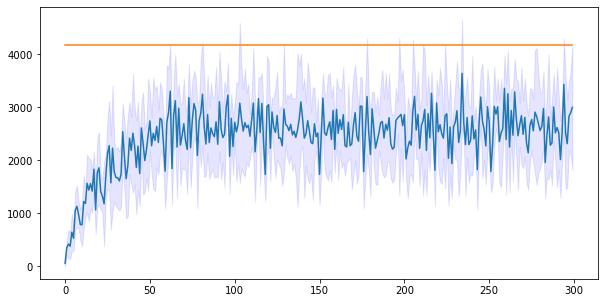
\includegraphics[width=0.5\textwidth]{img/reward2.png}
        \caption{Reward}
        \label{fig:reward2}
        \end{center}
    \end{figure}
    \columnbreak
As said before here we can see\\ that the algorithm converge to a solution\\ that is not optimal,\\ so return a reward that is lower \\than the best possible one (clairvoyant)
\end{multicols}

\begin{multicols}{2}
    \begin{figure}[H]
        \begin{center}
        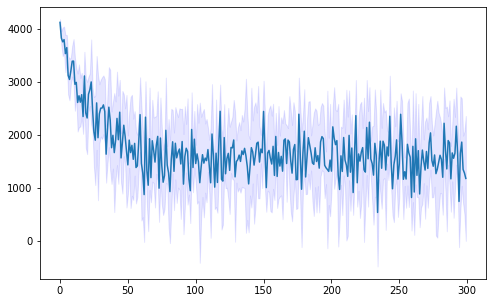
\includegraphics[width=0.5\textwidth]{img/regret2.png}
        \caption{Regret}
        \label{fig:regret2}
        \end{center}
    \end{figure}
    \columnbreak
    \begin{figure}[H]
        \begin{center}
        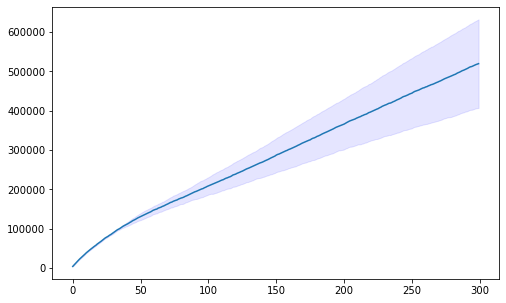
\includegraphics[width=0.5\textwidth]{img/cum_regret2.png}
        \caption{Cumulative regret}
        \label{fig:cum_reg2}
        \end{center}
    \end{figure}
\end{multicols}
As expected the cumulative reward is linear (Figure 3)
